\documentclass[aspectratio=169]{beamer}
\usetheme{Madrid}
\usepackage{graphicx}
\usepackage{array}

\title{GemmaScope Position/Budget Checkpoint}
\subtitle{Model merging SAE project}
\author{Local research log}
\date{2026-05-22}

\newcommand{\smallcode}[1]{\texttt{\scriptsize #1}}

\begin{document}

\begin{frame}
  \titlepage
  \vspace{-0.6cm}
  \begin{center}
    Checkpoint reason: position-restricted sparse repair is stable enough to move into feature-ID causality.
  \end{center}
\end{frame}

\begin{frame}{Plain Definitions}
  \begin{itemize}
    \item Model merging combines model weights or task deltas. In this project, the merge/abliteration damaged refusal behavior.
    \item A sparse autoencoder (SAE) gives sparse feature coordinates that reconstruct Gemma-2-2B MLP activations.
    \item A patch replaces selected recipient activations with donor-like decoded SAE contributions.
    \item A position mask asks where the patch must be applied: harmful prompt content, assistant/template boundary tokens, generated tokens, or combinations.
  \end{itemize}
\end{frame}

\begin{frame}{Current RQ}
  \textbf{Question:} do the selected GemmaScope MLP-SAE features repair refusal because they encode harmful-content semantics, or because they restore a response-start/refusal-state trajectory?

  \vspace{0.35cm}
  \textbf{Why it matters:}
  \begin{itemize}
    \item A content-feature story would support semantic feature interpretation.
    \item A trajectory-state story is still mechanistic, but it points to response initialization and rollout maintenance as the merge failure.
    \item The next feature-level experiment should target the correct causal path.
  \end{itemize}
\end{frame}

\begin{frame}{Key Aggregate Table}
  \scriptsize
  Cells are harmful clean refusal / unsafe continuation. Benign helpfulness is 1.00 for all listed rows.

  \vspace{0.15cm}
  \begin{tabular}{>{\raggedright\arraybackslash}p{1.15cm}p{0.85cm}p{1.55cm}p{1.9cm}p{1.75cm}p{1.85cm}}
    \hline
    Budget & Fold & All pos & Boundary+gen & Content+gen & Template+gen \\
    \hline
    k1024 & 4:8 & 1.00 / 0.00 & 0.75 / 0.00 & 0.00 / 0.00 & 0.75 / 0.00 \\
    k1024 & 8:12 & 0.75 / 0.00 & 0.75 / 0.00 & 0.00 / 0.00 & 0.75 / 0.00 \\
    k2048 & 4:8 & 1.00 / 0.00 & 0.75 / 0.00 & 0.25 / 0.25 & 0.75 / 0.00 \\
    k2048 & 8:12 & 0.75 / 0.00 & 0.75 / 0.25 & missing & 0.75 / 0.25 \\
    k512 & 4:8 & -- & 0.75 / 0.00 & -- & -- \\
    k512 & 8:12 & -- & 0.50 / 0.00 & -- & -- \\
    \hline
  \end{tabular}
\end{frame}

\begin{frame}{Plot View}
  \begin{center}
    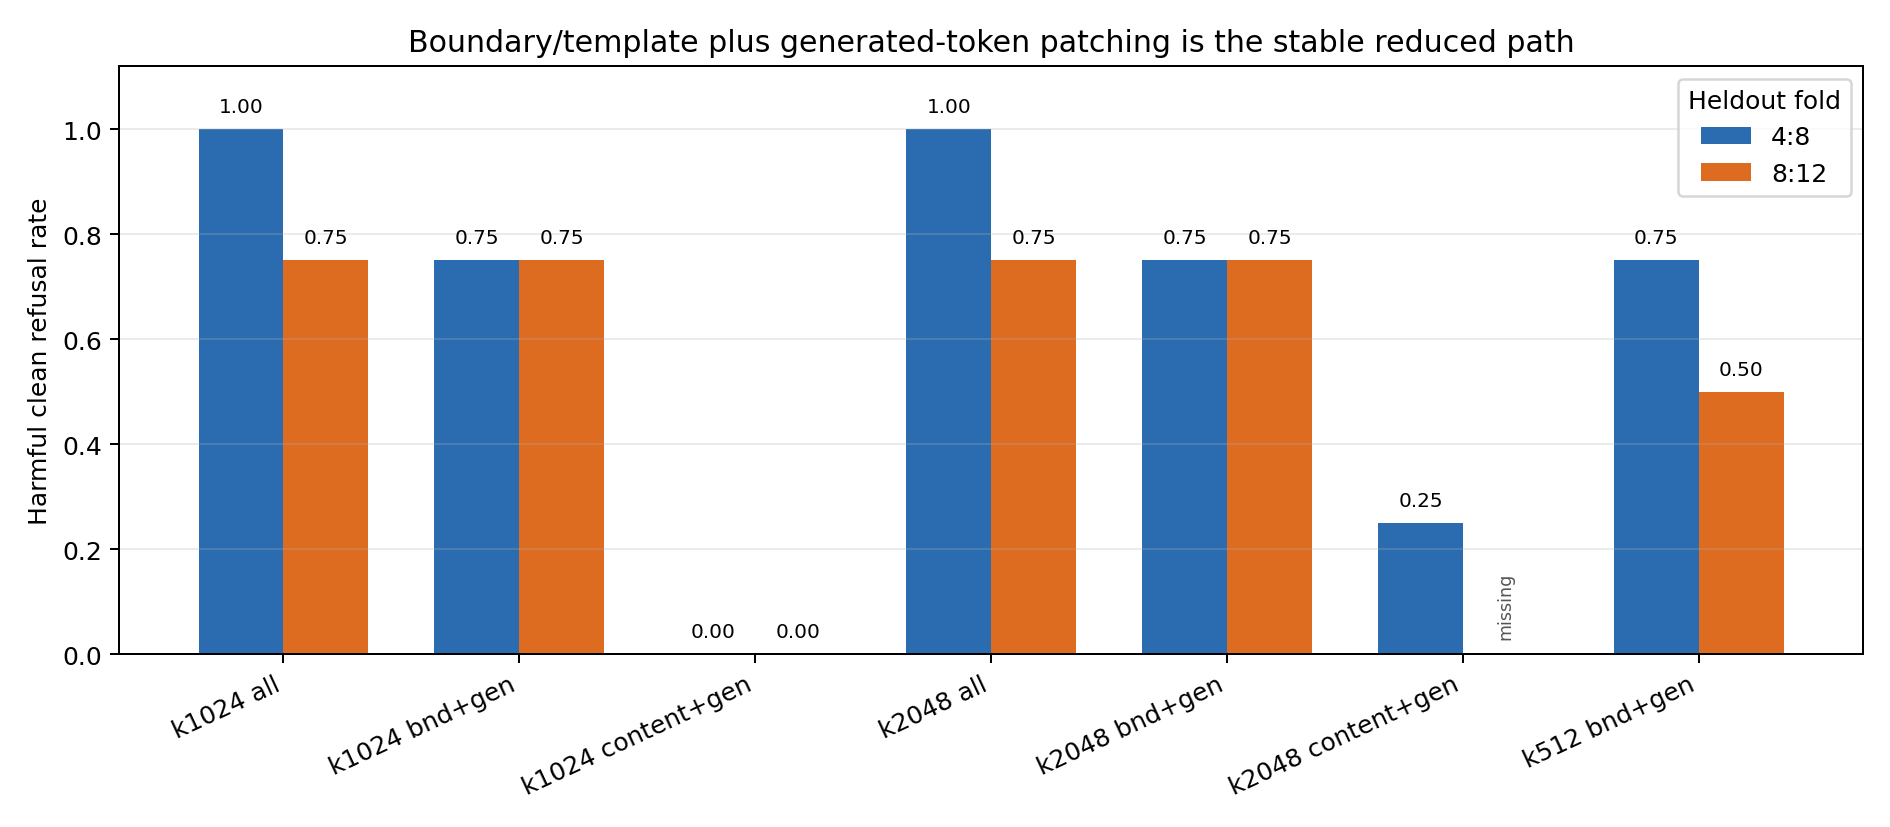
\includegraphics[width=0.93\textwidth]{figures/position_budget_harmful_clean.png}
  \end{center}
  \vspace{-0.2cm}
  \scriptsize Boundary/template plus generated-token patching is the stable reduced path; content+generated stays weak and noisy.
\end{frame}

\begin{frame}{Interpretation}
  \begin{itemize}
    \item Static assistant-boundary-only patching fails, so the mechanism is not just one prompt token being overwritten.
    \item Generated-token-only patching also fails, so rollout maintenance needs a prompt-side seed.
    \item \smallcode{assistant\_boundary\_or\_generated} and \smallcode{prompt\_template\_or\_generated} are the best reduced paths.
    \item k2048 does not make content+generated competitive; it adds weak repair plus unsafe continuation.
    \item k512 remains partially causal, so k1024 is not just an overlarge accidental feature set.
  \end{itemize}
\end{frame}

\begin{frame}{Decision And Next Step}
  \textbf{Decision:} keep the project. This is now a plausible mechanistic claim, but it is not feature-level yet.

  \vspace{0.35cm}
  \textbf{Next experiment:}
  \begin{itemize}
    \item Move from position masks to feature-ID causality inside the boundary/template plus generated-token path.
    \item Ablate or isolate top features by layer and generated-token time slice.
    \item Test whether a compact feature bundle carries refusal-state setup and maintenance.
  \end{itemize}
\end{frame}

\begin{frame}{Provenance}
  \scriptsize
  \begin{itemize}
    \item k1024: \smallcode{stage3/results/gemma2\_2b\_gemmascope\_mlp\_sae\_position\_restricted\_atomic\_v0/}
    \item k2048: \smallcode{stage3/results/gemma2\_2b\_gemmascope\_mlp\_sae\_position\_restricted\_k2048\_v0/}
    \item k512 budget: \smallcode{stage3/results/gemma2\_2b\_gemmascope\_mlp\_sae\_boundary\_generated\_budget\_v0/}
    \item Aggregator: \smallcode{stage3/scripts/aggregate\_gemma2\_2b\_gemmascope\_mlp\_sae\_position\_restricted.py}
    \item Copied deck data: \smallcode{presentations/2026-05-22-1717-gemmascope-position-budget/data/}
  \end{itemize}
\end{frame}

\end{document}
